\chapter{Vorauslegung}
\label{chap:Vorauslegung}
% Ziel hier: den Leser in die Lage versetzen, die wesentliche Struktur der Arbeit nachvollziehen zu können (Vorgehen / Geräte / Materialien / Verfahren [also auch Software]  / getroffene Annahmen ... sollten hier erklärt werden)
Die Flugdaten kommen aus einer Trajektoriensimulation aus dem Simulationsprogramm OpenRocket, welche vom Triebwerk-Subsystem durchgeführt wurde.
Diese Flugdaten~(\ref{fig:flugdaten_trajektoriensimulation}) sind eine Maximalabschätzung der Schubkraft und Dauer mit \SI{8}{\kilo\newton} für \SI{43}{\second},
welche in maximaler Flugdauer und Aerodynamischen Aufheizung resultieren.

\section{Anforderungen}

Da die Kühlung zeitgleich zu der Avionik entwickelt wurde, musste auf eine genaue Analyse aller Komponenten der Avionik verzichtet werden.
Stattdessen wurde anhand des bereits festgelegten Microcontrollers STM32H743ZGT6, der auf den redundanten Flugcomputern verwendet wird,
die Auslegung durchgeführt.
Aus dem Datenblatt des Microcontrollers folg eine maximale Sperrschichttemperatur von $T_\text{J} = \SI{125}{\degreeCelsius}$~\cite{STM32}
und ein Sperrschicht-Gehäuse Wärmeleitwiederstand von $\Theta_\text{JC} = \SI{23.9}{\degreeCelsius\per\watt}$~\cite{STM32}. Mit einem konservativen
Sicherheitsfaktor von 1.5, um bisher unbekannte Bauteile zu berücksichtigen, folgt daraus $\Theta_\text{JC,safety} = \SI{35.85}{\degreeCelsius\per\watt}$
und eine maximale Gehäusetemperatur von $T_\text{C} = \SI{89.15}{\degreeCelsius}$. Im Kontext der Elektronik ist mit Gehäuse immer die
Oberseite der elektronischen Komponente gemeint.
Die Kühlung soll außerdem eine hohe Zuverlässigkeit haben, welche durch Verwendung von ausschließlich passiven Bauteilen gewehrleistet wird.
Dadurch kann aufwendiges und teures testen und verifizieren von aktiven Bauteilen mit mechanischer oder elektrischer Funktion vermieden werden und es besteht bei
nicht nominalen Flügen eine geringere Ausfallwahrscheinlichkeit durch die inherent größeren Toleranzen passiver Bauteile.

Dem Energieerhaltungssatz nach haben der \ac{fcc}, die Kameras und weitere Elektronik die keine Leistung abgibt, gegenüber etwa
der \ac{pcdu} und Funkplatine welche Leistung in Form von Strom und elektromagnetischer Strahlung abgeben, einen Wirkungsgrad von
\SI{0}{\percent}, da Logikoperationen physikalisch gesehen keine Arbeit sind. Resultierend wird der komplette Stromverbrauch
in Wärme umgewandelt.

\begin{table}[H]
  \centering
  \caption{Leistung der Avionik}\label{tab:avionik_leistung}

  \begin{tabular}{lp{4cm}ll}
    \toprule[1pt]
    Komponente & Spannung \& Strom & Wirkungsgrad & Wärmestrom \\
    \midrule[0.5pt]

    STM32H743ZGT6 &
      \mbox{$V_\text{DD}=\SI{3.3}{\volt}$},\newline
      $I_\text{DD}=\SI{536}{\milli\ampere}$~\cite{STM32} &
      $\approx \SI{0}{\percent}$ & \SI{1.769}{\watt} \\
    $\dot{Q}_\text{ges}$ & & & \SI{7.075}{\watt}\\

    \midrule[0.5pt]
    RunCam Split 4 V2 &
      \mbox{$V_\text{DD}=\SI{5}{\volt}$},\newline
      $I_\text{DD}=\SI{450}{\milli\ampere}$~\cite{RunCam-Split4V2} &
      $\approx \SI{0}{\percent}$ & \SI{2.25}{\watt} \\
    $\dot{Q}_\text{ges}$ & & & \SI{9}{\watt}\\

    \midrule[0.5pt]
    Thebe-II &
      \mbox{$V_\text{DD}=\SI{3.6}{\volt}$},\newline
      $I_\text{DD}=\SI{500}{\milli\ampere}$~\cite{WE-ThebeII-UM-2024} &
      $\approx \SI{30}{\percent}$~\cite{WE-ThebeII-UM-2024} & \SI{1.3}{\watt} \\

    \midrule[0.5pt]
    \ac{pcdu} & & $\approx \SI{30}{\percent}$ & \SI{9.3}{\watt} \\

    \midrule[0.5pt]
    \midrule[0.5pt]
    $\dot{Q}_\text{ges, safety}$ & & & \SI{40}{\watt} \\

    \bottomrule[1pt]
  \end{tabular}
\end{table}

Die Leistung der Avionik~\ref{tab:avionik_leistung} ergibt sich durch den Maximalverbrauch der \ac{fcc} mikrocontroller bei maximaler clock rate
(\SI{400}{\mega\hertz}) und vollständig aktiver Peripherie, der Kameras und einer Abschätzung der restlichen Komponenten ohne Quellenangabe.
Der aus \ref{tab:avionik_leistung} resultierende gesamten Wärmestrom der Avionik mit \SI{40}{\watt} ist mit einem gewöhnlichen Laptop vergleichbar.

\begin{figure}[H]
    \centering

    % Column 1, Row 1
    \begin{subfigure}{0.48\textwidth}
        \centering
        \includegraphics[width=\linewidth]{../../Code/acceleration_over_time.pdf}
        \caption{Beschleunigung während Flug}
        \label{fig:acceleration_over_time}
    \end{subfigure}
    \hfill
    % Column 2, Row 1
    \begin{subfigure}{0.48\textwidth}
        \centering
        \includegraphics[width=\linewidth]{../../Code/altitude_over_time.pdf}
        \caption{Flughöhe}
        \label{fig:altitude_over_time}
    \end{subfigure}

    \vspace{1em}

    % Column 1, Row 2
    \begin{subfigure}{0.48\textwidth}
        \centering
        \includegraphics[width=\linewidth]{../../Code/pressure_over_time.pdf}
        \caption{Statischer Luftdruck während Flug}
        \label{fig:pressure_over_time}
    \end{subfigure}
    \hfill
    % Column 2, Row 2
    \begin{subfigure}{0.48\textwidth}
        \centering
        \includegraphics[width=\linewidth]{../../Code/temperature_over_time.pdf}
        \caption{Statische Lufttemperatur während Flug}
        \label{fig:temperature_over_time}
    \end{subfigure}

    \vspace{1em}

    % Column 1, Row 3
    \begin{subfigure}{0.48\textwidth}
        \centering
        \includegraphics[width=\linewidth]{../../Code/velocity_over_time.pdf}
        \caption{Geschwindigkeit während Flug}
        \label{fig:velocity_over_time}
    \end{subfigure}
    \hfill
    % Column 2, Row 3
    \begin{subfigure}{0.48\textwidth}
        \centering
        \includegraphics[width=\linewidth]{../../Code/dynp_during_flight.pdf}
        \caption{Dynamischer Druck während Flug}
        \label{fig:dynp_over_time}
    \end{subfigure}

    \caption{Flugdaten der Trajektoriensimulation}\label{fig:flugdaten_trajektoriensimulation}
\end{figure}

\section{Thermales Interface}\label{thermalesInterface}

\subsection{Heatpipes}

Hetpipes sind super

\subsection{Thermal Straps}\label{thermalstraps}

Um das \ac{pcb} mit der Heatpipe zu verbinden werden Thermal Straps aus verschiedenen Materialien analysiert.
Thermal Straps sind flexible Verbindungsteile die Wärmebrücken zwischen mehreren Bauteilen gewehrleisten.
Wegen der hohe Wärmeleitzahl von \ac{pgs} und bedonders für Thermal Straps wichtigen Flexibilität, sind diese eine interessante Option.
Ein Nachteil von \ac{pgs} ist die geringe Dicke und der daraus resultierende geringe Querschnitt, welcher trotz hoher Wärmeleitzahl zu hoher Wärmestromdichte und stärkerer Temperaturerhöhung führen kann.
Im Vergleich mit herkömmlichen Materialien wie Aluminium und Kupfer soll ein Vergleich gezogen werden.

\begin{figure}[H]
  \centering
  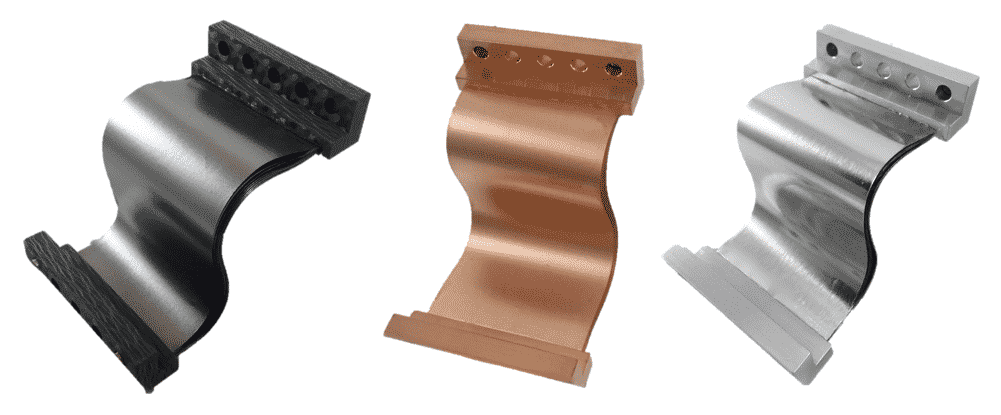
\includegraphics[width=\textwidth]{thermal_straps_commercial.png}
  \caption{Kommerzeill erhältliche Thermal Straps aus Graphen, Kupfer und Aluminium~\cite{Thermal-Straps}}\label{fig:thermalstraps_commercial}
\end{figure}

\section{Phase Change Materials}\label{sec:pcm}

\ac{pcm} mit Fest-Flüssig Übergang sind eine weit verbreitete Lösung in der Luft- und Raumfahrtindustrie um für für begrenzte Zeiträume Elektronik in einem akzeptablen
Temperaturbereich zu halten. Auch wenn \ac{pcm} Lösungen generell eine hohe Masse haben, wird das oft aufgrund der ansonsten idealen Eigenschaften inkauf genommen.
Durch die hohe spezifische Schmelzenthalpie, kann rein passiv eine große Wärmemenge, bei einem isothermen Prozess, absorbiert werden. Aufgrund dessen
kann ein von der Umwelt isoliertes \ac{atm} entwickelt werden, das nicht mit stark schwankenden Zuständen der Sonneneinstrahlung und Lufttemperatur
zurecht kommen muss. Auch wenn \ac{pcm} im Flüssig-Gas Übergang meist eine etwa 10-fach höhere Verdampfungsenthalpie haben, werden diese
generell nicht verwendet, da der Dichteunterschied zwischen Flüssig- und Gasphase zu extremen Drücken führen würden, falls Wiederverwendbarkeit
verlangt wird und somit ein Druckkörper nötig ist. Alternativ kann die Gasphase auch aus dem Fahrzeug abgelassen werden in einem Prozess der
Vapour Venting genannt wird. Hierbei geht jedoch die Wiederverwendbarkeit verloren, da vor jedem Start die Flüssigphase neu getankt werden muss.
Weiter kann das Venting trotz der geringen Massenströme zu Momenten führen, die das Fahrzeug destabilisieren; besonders im Überschallbereich
können unintuitive Momente entstehen~\cite{Deere-2011}, die aufwendige \ac{cfd}-Simulationen oder Tests benötigen. Dementsprechend wird nur ein
Fest-Flüssig \ac{pcm} analysiert.\\

Für die Auswahl eines geeigneten \ac{pcm} sind spezifische Schmelzenthalpie, Schmelztemperatur und Wärmeleitfähigkeit am wichtigsten.
Letzteres kann jedoch durch Lamellen oder ähnliche Strukturen, zur Verbesserung der Wärmeleitfähigkeit durch das komplette \ac{pcm} verbessert werden,
wobei dabei \ac{pcm} Masse mit Strukturmasse ersetzt wird und somit die Wärmekapazität verringert. Das Volumen der Wärmeleitenden Struktur welches
\ac{pcm} ersetzt wird Void Fraction genannt, da es gewissermaßen eine Leerstelle im \ac{pcm} bildet, die keine latente Wärmeaufnahme hat. Hier
wird ein Void Fraction von $F = 0.1$ todo

Die Thermodynamischen Eigenschaften von Eicosane, aufgeführt in Tabelle \ref{tab:eicosane_data}, wurden aus mehreren Quellen entnommen.\\

\begin{table}[H]

  \centering
  \caption{Stoffdaten für Eicosane}\label{tab:eicosane_data}

  \begin{tabular}{lll}

    \toprule[1pt]
    Solidus Temperatur & $T_{\text{solidus}}$ & \SI{309}{\kelvin}~\cite{NIST} \\

    \midrule[0.5pt]
    Liquidus Temperatur & $T_{\text{liquidus}}$ & \SI{311}{\kelvin}~\cite{NIST} \\

    \midrule[0.5pt]
    Spezifische Wärmekapazität bei\\konstantem Druck der\\Flüssigphase & $c_{p,\text{liquid}}$ & \SI{2350.05}{\joule\per\kilogram\per\kelvin}~\cite{NIST} \\

    \midrule[0.5pt]
    Spezifische Wärmekapazität bei\\konstantem Druck der\\Feststoffphase & $c_{p,\text{solid}}$ & \SI{2132.4}{\joule\per\kilogram\per\kelvin}~\cite{NIST} \\

    \midrule[0.5pt]
    Dichte der Flüssigphase & $\rho_{\text{solid}}$ & \SI{910}{\kilogram\per\cubic\meter}~\cite{Nazarychev-2022} \\

    \midrule[0.5pt]
    Dichte der Feststoffphase & $\rho_{\text{liquid}}$ & \SI{769}{\kilogram\per\cubic\meter}~\cite{Nazarychev-2022} \\

    \midrule[0.5pt]
    Wärmeleitfähigkeit der Flüssigphase & $\lambda_{\text{liquid}}$ & \SI{0.1505}{\watt\per\meter\per\kelvin}~\cite{Benbrika-2020} \\

    \midrule[0.5pt]
    Wärmeleitfähigkeit der Feststoffphase & $\lambda_{\text{solid}}$ & \SI{0.4248}{\watt\per\meter\per\kelvin}~\cite{Stryker-1990} \\

    \midrule[0.5pt]
    Wärmeausdehnungskoeffizient & $\gamma$ & \SI{0.0009}{\per\kelvin}~\cite{Benbrika-2020} \\

    \midrule[0.5pt]
    Spezifische Schmelzenthalpie & $h_{\text{fus}}$ & \SI{240998.86}{\joule\per\kilogram}~\cite{NIST} \\

    \bottomrule[1pt]
  \end{tabular}
\end{table}

\begin{lstlisting}[language=Python, caption={Berechnung der Masse und Latenten Wärmekapazität des \ac{pcm} in der pcm.py}, label={lst:pcm_masse_kapazität}]
rho_alu = 2700     # aluminium density [kg*m^-3]
rho_pcm = 788      # pcm density [kg*m^-3]
h      = 240998.9  # pcm latent heat [J*kg^-1]
F       = 0.1      # void fraction
t       = 0.001    # wall thickness [m]

def total_mass(L, H): # pcm mass including case and fins
    return (rho_alu * (L**2 * H - (L - 2*t)**2 * (H - 2*t))
            + (F * rho_alu + (1 - F) * rho_pcm) * (L - 2*t)**2 * (H - 2*t)) 

def total_heat(L, H): # pcm latent heat capacity
    #...#
    pcm_heat  = (1 - F) * rho_pcm * (L - 2*t)**2 * (H - 2*t) * h
    return pcm_heat
\end{lstlisting}

\begin{figure}[H]
    \centering
    \begin{subfigure}{0.9\textwidth}
        \centering
        \includegraphics[width=\linewidth]{../../Code/pcm_mass.pdf}
        \caption{PCM Masse}\label{fig:pcm_mass}
    \end{subfigure}
    \vspace{1em}  % Optional vertical spacing
    \begin{subfigure}{0.9\textwidth}
        \centering
        \includegraphics[width=\linewidth]{../../Code/pcm_heat_capacity.pdf}
        \caption{PCM Wärmeaufnahme}\label{fig:pcm_heat}
    \end{subfigure}
    \caption{PCM Auslegung}\label{fig:pcm_mass_heat}
\end{figure}

\newpage

\section{Radiator}\label{sec:Radiator}

Bei Radiatoren ist ein hoher Emissions- und niedriger Absorptionsgrad nach \ref{eq:radiation} dimensionierend, da die Temperatur den Anforderungen nach limitiert ist
und die Fläche minimiert werden muss, da diese proportional zu eingehende Wärmeströmen aus der Umgebung ist, welche auch möglichst gering gehalten werden müssen.\\
Als Beschichtung wurde AZ-93 der Firma AZ Technology LLC.~\cite{AZ-Technology} ausgewählt. Dabei handelt es sich um eine in der Raumfahrt
weit verbreitete inorganische Farbe mit idealen Eigenschaften, welche Tabelle \ref{tab:az-93_eigenschaften} entnommen werden können.
In \ref{fig:radiator_flaeche_leistung} sieht man für die ausgewählte Beschichtung die Leistung eines Radiators bei gegebener Temperatur und Fläche.
Durch in \ref{sec:pcm_radiator_hybrid} analysierte Wärmeströme, würde es bei nutzung eines einfachen Radiators schnell zur Überhitzung der Avionik kommen.\\


\begin{table}[H]

  \centering
  \caption{AZ-93 Spezifikationen~\cite{AZ-Technology}}\label{tab:az-93_eigenschaften}

  \begin{tabular}{ll}

    \toprule[1pt]
    $\epsilon_{\text{t}}$ & $0.91 \pm 0.02$ \\

    \midrule[0.5pt]
    $\alpha_{\text{s}}$ & $0.15 \pm 0.02$ \\

    \midrule[0.5pt]
    Temperaturbereich  & \SI{-180}{\degreeCelsius} bis \SI{1400}{\degreeCelsius} \\

    \bottomrule[1pt]
  \end{tabular}
\end{table}

\begin{figure}[H]
  \centering
  \includegraphics[width=\linewidth]{../../Code/radiator_leistung.pdf}
  \caption{Radiator Leistung nach Fläche und Temperatur}\label{fig:radiator_flaeche_leistung}
\end{figure}

\newpage

\section{PCM-Radiator-Hybrid}\label{sec:pcm_radiator_hybrid}

Eine Hybridlösung wird auch in erwägung gezogen, um die Masse durch Nutzung eines Radiators zu minimieren, wobei wegen aerodynamischer Aufheizung für kurze Zeit ein PCM gebraucht werden könnte.
Um eine umständliche Simulation mittels \ac{cfd} zu vermeiden, wird die Außenkontour der Rakete von Spitze bis Avionik-Sektion, mit Hilfe der Nußelt-Beziehungen, als längsangeströmte ebene Platte angesehen,
wie in Abbildung~\ref{fig:rakete_kontour_zeichnung} dargestellt ist.
Um zu wissen, ob hier die Beziehung für laminare oder turbulente Grenzschichten angewandt werden soll, müssen zunächst die Gültigkeitsbereiche der Reynolds- und Prandtlzahl (\ref{eq:prandtl},~\ref{eq:reynolds}) überprüft werden.
Mittels der Nußelt-Beziehung wird $\alpha$ bestimmt und dann in Gleichung~\ref{eq:qdot} eingesetzt, um auf den spezifischen Wärmestrom zu schließen.

\newpage
% Hybrid PCM ohne aufheizung

\begin{figure}
  \centering
  \begin{tikzpicture}[rotate border/.style={shape border uses incircle, shape border rotate=#1}, scale=0.8]
    \draw[thick] (3,3) -- (3,-1) -- (9,-1) -- (9,3);
    \draw[thick] (3,3) -- node [midway, above] {Avionik Sektion}  (9,3);
    \draw[thick] (4,3) -- (4,-1); % PCM Lamellen
    \draw[thick] (3,-0.5) -- (4,-0.5);
    \draw[thick] (3,0) -- (4,0);
    \draw[thick] (3,0.5) -- (4,0.5);
    \draw[thick] (3,1) -- (4,1);
    \draw[thick] (3,1.5) -- (4,1.5);
    \draw[thick] (3,2) -- (4,2);
    \draw[thick] (3,2.5) -- (4,2.5);
    \node at (-0.5,2) [style={single arrow, draw}, minimum height=3cm, minimum width=0.5cm, thick]{$\dot{Q}_{\mathrm{Umwelt}}$}; % Wärmestrom pfeil
    \node at (-0.5,0) [style={single arrow, draw}, minimum height=4.5cm, minimum width=1.5cm, shape border rotate=180, thick]{$\dot{Q}_{\mathrm{Radiator}}$}; % Wärmestrom pfeil
    \node at (6.5,1)[style={single arrow, draw}, minimum height=3cm, minimum width=0.5cm, shape border rotate=180, thick]{$\dot{Q}_{\mathrm{Avionik}}$}; % Wärmestrom pfeil
    \draw[->, thick, -{Stealth[length=0.25cm]}] (1,3.75) node [above=1pt] {PCM mit Lamellen} -- (3.5,2.6);
  \end{tikzpicture}
  \caption{PCM Wärmestrom ohne aerodynamische Aufheizung}\label{fig:pcm_waermestrom_diagramm}
\end{figure}

$\dot{Q}_{\mathrm{Radiator}} = \dot{Q}_{\mathrm{Umwelt}} + \dot{Q}_{\mathrm{Avionik}}$ In diesem Fall reicht die Leistung des Radiators, um die Avionik auf Betriebstemperatur zu halten.
% Hybrid PCM Wärmestrom bei aufheizung

\begin{figure}[H]
  \centering
  \begin{tikzpicture}[rotate border/.style={shape border uses incircle, shape border rotate=#1}, scale=0.8]
    \draw[thick] (3,3) -- (3,-1) -- (9,-1) -- (9,3);
    \draw[thick] (3,3) -- node [midway, above] {Avionik Sektion}  (9,3);
    \draw[thick] (4,3) -- (4,-1); % PCM lamellen
    \draw[thick] (3,-0.5) -- (4,-0.5);
    \draw[thick] (3,0) -- (4,0);
    \draw[thick] (3,0.5) -- (4,0.5);
    \draw[thick] (3,1) -- (4,1);
    \draw[thick] (3,1.5) -- (4,1.5);
    \draw[thick] (3,2) -- (4,2);
    \draw[thick] (3,2.5) -- (4,2.5);
    \node at (-0.5,2) [style={single arrow, draw}, minimum height=4.5cm, minimum width=1.5cm, thick]{$\dot{Q}_{\mathrm{Umgebung}}$}; % Wärmestrom pfeil
    \node at (-0.5,0) [style={single arrow, draw}, minimum height=4.5cm, minimum width=1.5cm, shape border rotate=180, thick]{$\dot{Q}_{\mathrm{Radiator}}$}; % Wärmestrom pfeil
    \node at (6.5,1)[style={single arrow, draw}, minimum height=3cm, minimum width=0.5cm, shape border rotate=180, thick]{$\dot{Q}_{\mathrm{Avionik}}$}; % Wärmestrom pfeil
  \end{tikzpicture}
  \caption{PCM Wärmestrom bei aerodynamischer Aufheizung}\label{fig:pcm_waermestrom_aufheizung_diagramm}
\end{figure}

Hier reicht die Leistung des Radiators nicht mehr aus und das \ac{pcm} fängt an zu schmilzen. Zu beachten ist,
dass die Leistung des Radiators durch die Temperaturerhöhung steigen würde, wegen des \ac{pcm} jedoch sehen wir das System als isotherm an.
% Raketenkontour im Luftstrom für ebene Platte Annahme

\begin{figure}[H]
  \centering
  \begin{tikzpicture}
    \draw[thick] (0,0) arc [start angle=90, end angle=270, x radius=5cm, y radius= 1.5cm]; %nosecone
    \draw[thick] (0,0) -- (3,0); % hülle
    \draw[thick] (0,-3) -- (3,-3); % hülle
    \draw[thick] (-5.75,-1.5) -- (-5.25,-1.5); % maß links
    \draw[thick] (1,0.25) -- (1,0.75); % maß rechts
    \draw[thick] (0,0.5) arc [start angle=90, end angle=180, x radius=5.5cm, y radius= 2cm]; % maß bogen
    \draw[thick] (0,0.5) -- node [near start, above] {Länge} (1,0.5); % maß grade sektion
    \draw[->, thick, -{Stealth[length=0.25cm]}] (-10,0.5) -- node [midway, above] {Luftstrom} (-7,0.5); % free stream pfeile
    \draw[->, thick, -{Stealth[length=0.25cm]}] (-10,-0.5) -- (-7,-0.5); % Strompfeile
    \draw[->, thick, -{Stealth[length=0.25cm]}] (-10,-1.5) -- (-7,-1.5);
    \draw[->, thick, -{Stealth[length=0.25cm]}] (-10,-2.5) -- (-7,-2.5);
    \draw[->, thick, -{Stealth[length=0.25cm]}] (-10,-3.5) -- (-7,-3.5);
    \draw[thick] (0,0) -- (0,-2.5); % casing wall
    \draw[thick] (2,0) -- (2,-2.5); % casing wall
    \draw[thick] (0,-2.5) -- (2,-2.5); % casing bottom
    \node at (1,-1.5) [style={single arrow, draw}, minimum height=0.5cm, minimum width=1.5cm, rotate=90, thick]{$\dot{Q}_{\mathrm{Avionik}}$}; % Wärmestrom pfeil
  \end{tikzpicture}
  \caption{Kontourlänge vom Staupunkt der Rakete bis zum Mittelpunkt des Radiators}\label{fig:rakete_kontour_zeichnung}
\end{figure}

In Abbildung~\ref{fig:dimensionierung_ablauf} sieht man wie die Dimensionierung in den Programmen abläuft. Die Programme erzeugen alle Graphen und rechnen simultan für gegebenen Avionik Wärmestrom alle Werte aus.

\begin{figure}[H]
  \centering
  \begin{tikzpicture}[
    sibling distance=10em,
    every node/.style = {
      shape=rectangle,
      rounded corners,
      draw,
      align=center,
      minimum width=3cm
    },
    edge from parent/.style = {
      draw,
      ->,
      -{Stealth[length=0.25cm]},
      thick
    },
    arrow/.style = {
      ->,
      -{Stealth[length=0.25cm]},
      thick
    }
  ]

    % Top nodes
    \node (avionik) at (-2.1, 4) {Avionik Wärmestrom};
    \node (sonne)   at ( 2.1, 4) {Sonne Wärmestrom};

    % Radiator Fläche centered below
    \node (radiator) at (0, 2) {Radiator Fläche};

    % Children of Radiator
    \node (breite) at (-2.1, 0) {PCM Breite};
    \node (aerothermal) at (2.1, 0) {Aerothermal Wärmestrom};

    % PCM Kapazität as a separate node (not a child directly)
    \node (kapazitaet) at (2.1, -2) {PCM Kapazität};

    % PCM Höhe node below the center of breite and kapazitaet
    \node (hoehe) at (0, -4) {PCM Höhe};
    \node (gewicht) at (0, -6) {PCM Gewicht};

    % Arrows
    \draw[arrow] (avionik) -- (radiator);
    \draw[arrow] (sonne) -- (radiator);
    \draw[arrow] (radiator) -- (breite);
    \draw[arrow] (radiator) -- (aerothermal);
    \draw[arrow] (aerothermal) -- (kapazitaet);
    \draw[arrow] (breite) -- (hoehe);
    \draw[arrow] (kapazitaet) -- (hoehe);
    \draw[arrow] (hoehe) -- (gewicht);

  \end{tikzpicture}
  \caption{Dimensionierungs-Ablauf in der Vorauslegung}\label{fig:dimensionierung_ablauf}
\end{figure}

\begin{figure}[H]
  \centering
  \includegraphics[width=\linewidth]{../../Code/re_pr_during_flight.pdf}\label{fig:re_pr_flugsimulation}
  \caption{Reynolds- und Prandtlzahl während kritischer Phase im Flug}
  \includegraphics[width=\linewidth]{../../Code/pcm_radiator_hybrid_heatflux_nosim.pdf}\label{fig:pcm_waermestrom_vorauslegung}
  \caption{PCM Wärmestrom während Flug}
\end{figure}